\subsection{Maquettes d'écran} \label{sec:maquettes_ecran}

\subsubsection{Présentation de la version initiale}
Une première version des maquettes a été réalisée avec une interface volontairement sobre, minimaliste et orientée vers un public adolescent ou adulte. 
Les écrans issus de cette itération sont consultables à la \autoref{sec:écrans_v1}.

Cette version permettait notamment à l'utilisateur de choisir son environnement de développement : programmation par blocs (\acrshort{vpl}) ou écriture directe de code dans une interface de type \acrfull{ide}. 
Un écran de configuration était également proposé afin de faciliter la connexion à un robot e-puck2.

\subsubsection{Présentation de la version améliorée}
La version finale s'inspire de la structure de la première, tout en introduisant plusieurs ajustements pour mieux correspondre aux attentes et besoins du public visé.

Afin de rendre l'application plus inclusive et attrayante, tant du point de vue du genre que de l'âge, plusieurs éléments ont été adaptés : une sélection de thèmes visuels plus variée (dont des palettes de couleurs plus mixtes comme le rose, des styles "Lego Mindset", "futuriste", ou encore "aventure"), une différenciation des écrans selon deux tranches d'âge (6–12 ans et 13–18 ans), et la possibilité de masquer l'affichage du code source derrière un bouton dédié, permettant ainsi de réduire la charge cognitive pour les plus jeunes.

Ces adaptations visent à offrir une interface plus accueillante pour les enfants, tout en répondant au défi de favoriser la participation des filles dans les domaines des \acrfull{stim}.

En termes d’expérience utilisateur, cette version suit une logique progressive inspirée des "assistants d'installation" utilisés dans de nombreux logiciels. 
L'utilisateur est guidé étape par étape, depuis la personnalisation de l’interface jusqu’à l’utilisation fonctionnelle du robot.

Le schéma présenté en \autoref{fig:app_usage_flow} illustre le parcours utilisateur typique au sein de l’application. 
Les \textbf{blocs jaunes} correspondent aux étapes de \textit{personnalisation de l'application}, permettant d'adapter l'expérience utilisateur en fonction de ses préférences et de son profil.
Le \textbf{bloc bleu} matérialise une \textit{décision structurante} qui détermine le comportement du robot et influence directement les interactions dans les écrans suivants.
Enfin, les \textbf{blocs verts} désignent les \textit{actions répétées et récurrentes} que l’utilisateur effectuera régulièrement au cours de ses sessions d'utilisation.

\begin{figure}[H]
    \centering
    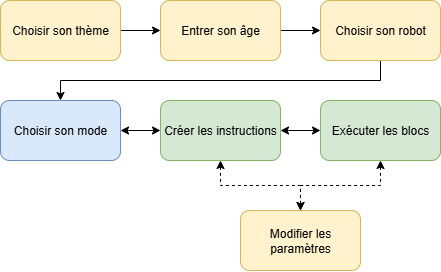
\includegraphics[width=0.75\linewidth]{.//figures//flow.png}
    \caption{\label{fig:app_usage_flow} Flux d'utilisation de l'application}
\end{figure}

